



\documentclass[journal]{IEEEtran}

\usepackage{cite}
\usepackage{graphicx}
\DeclareGraphicsExtensions{.pdf,.jpeg,.png}
\usepackage{amsmath}
\interdisplaylinepenalty=2500
\usepackage{array}
\usepackage{fixltx2e}
\usepackage{url}


% correct bad hyphenation here
\hyphenation{op-tical net-works semi-conduc-tor}


\begin{document}
% Definition of blocks:

\title{EEG and MEG Inversion Using Convolutional and Recurrent Neural Networks}


\author{Joaquin~J.~Casanova,~\IEEEmembership{Member,~IEEE,}
        Zachary~D.~Stoecker-Sylvia,
        Ryan~Y.~Miyamoto,~\IEEEmembership{Member,~IEEE,}
        and~Jenshan~Lin,~\IEEEmembership{Fellow,~IEEE}% <-this % stops a space
\thanks{J. Casanova and J. Lin are with the Department
of Electrical and Computer Engineering, University of Florida, Gainesville,
FL, 32611 USA e-mail: jcasa@ufl.edu}% <-this % stops a space
\thanks{R. Miyamoto and Z. Stoecker-Sylvia are with Oceanit.}% <-this % stops a space

\thanks{Manuscript received }}

% The paper headers
\markboth{Transactions on Medical Imaging,~Vol.~XX, No. YY}%
{Casanova \MakeLowercase{\textit{et al.}}: EEG and MEG Dipole Localization Using Convolutional and Recurrent Neural Networks}
\maketitle

\begin{abstract}

  Real-time localzation of neuronal activity has a number of uses, including brain-computer interfaces and medical diagnostics. Generally, this is done by taking measurements of the brain's magnetic and electric fields (magnetoencephalography [MEG] and electroencephalography [EEG]), and inverting the measurements. Most approaches are physics-based, and attempt to find the best estimate of the lead-field matrix, which relates the dipole activation to the field strength by minimizing the error of an estimate. To date, most approaches using the lead-field matrix are complicated and too slow in real time, aimed primarily at elucidating brain structural functional relationships from experimental data. We propose a new technique in which the location of peak neuronal current is estimated by treating EEG and MEG as a two-channel image, or time-series of images, which is processed by a neural network which returns the location of the dipole of peak magnitude. Four archtectures are tested: 2-layer perceptron, convolutional neural network (CNN), recurrent neural network (RNN), and CNN feeding RNN. In the absence of true measures of neuronal activity, we used two publicly available MEG/EEG datasets, and treated the estimates of the traditional minimum-norm estimate (MNE) as true estimates. We test the four variations of the network architecture, and in the best case (CNN only), we achieve test dataset errors (RMSE of max dipole location) of 1.9 and 5.1 mm on two separate datasets of MEG/EEG timeseries from subjects with different types of stimulus.
  
\end{abstract}

% Note that keywords are not normally used for peerreview papers.
\begin{IEEEkeywords}
EEG, MEG, Localization, Neural networks.
\end{IEEEkeywords}



\IEEEpeerreviewmaketitle



\section{Introduction}

\IEEEPARstart{T}{here} is a great need for interpretation of brain signals for both use in control of devices, for prosthetics, for example, or for disease diagnostics. Magnetoencephalography (MEG), the measurement of the brain's magnetic field, is typically done using cryogenic superconducting quantum interference devices (SQUID) on a dense grid surrounding the skull, and has been used in brain-computer interfaces \cite{mellinger2007meg}. Additionally, electroencephalography (EEG), is also used for BCI as well as medical diagnostics and study of brain stucture and function \cite{da2008impact}. Particularly for the latter, there is great utility in using the external measurements of MEG and EEG to determine which parts of the brain are most electrically active, a problem known as localization or inversion. Functional magnetic resonance imaging (fMRI) can be used but instead measures blood flow, and is thus not a direct measurement of electrical activity \cite{sharon2007advantage}.


Classically, MEG/EEG inversion has followed one of a few approaches, with incremental enhancements as sophistication and computational power has increased. \cite{grech2008review} provides an excellent review of techniques. \cite{mosher1992multiple} established the orignal framework of the dipole in a sphere model, in which a lead-field matrix based on magnetostatic and electrostatic equations, and the positions of dipoles, transforms a vector of dipole magnitudes into a vector of magnetic flux and electric potential at sensor locations. The problem of localization becomes a problem of finding the locations and magnitudes of dipoles that minimize the square error of predicted versus observed fields. Using this formalism and a finite-element model, \cite{buchner1997inverse} localized dipoles from MEG data. \cite{galka2004solution} used Kalman filtering to solve the dynamical inverse problem. The signal-space separation method transforms the data into basis functions in signal space to better filter background noise sources \cite{taulu2005applications}. Beamformer techniques have also been applied for MEG/EEG inversion \cite{sekihara2001reconstructing}. More recently, EEG has been inverted using artificial neural networks \cite{van2000eeg}.


Neural networks have proven an important tool for accurate predictions from noisy and large datasets. A recent technique is convolutional neural networks, in which image inputs are convolved with weighted kernels \cite{lecun1998gradient}. To treat time-series or sequences, recurrent neural networks, incorporating temporal feedback, have been developed, such as the long-short-term memory RNN \cite{hochreiter1997long}. CNN and RNN have been combined in \cite{venugopalan2014translating} to translate video sequences into text descriptions of the video.


Our proposed idea is to apply the combined CNN/RNN framework to sequences of MEG/EEG data, and predict the location of only the peak dipole. In this way we simplify the problem, and with approporiately trained networks, we could make quick predicts from data, possibly in real time. To demonstrate our technique, we use publicly available datasets, and use the dipole currents predicted by a well established technique (MNE) as the true value to which we compare our estimates and train our network \cite{gramfort2014mne}. Further, we investigate four variations of the network architecture (2-layer MLP, RNN, CNN, and CNN with RNN), to establish the advantages and disadvantages of each.

\section{Methods}

In this section, we describe our methodology, including datasets, preprocessing, and neural network architectures.

\subsubsection{Datasets}

To test our method, we used two multimodal datasets. Both were processed using the python-mne package \cite{gramfort2014mne}.

One dataset \cite{wakeman2015multi} consisted of 19 subjects presented with stimulus of famous, unfamiliar, or scrambled faces. There were 102 magnetometers, 204 planar gradiometers, and 70 electrodes, with 3 electrodes used for ocular and cardiac arifacts. We excluded gradiometers, as our study is to develop an inversion technique for use with our own MEG system, which only has the radial magnetometers. We considered one subject only (sub007) as that subject's MRI was the only one to segment properly into skin, skull, and cortex layers (an important feature for the inversion step). We used the data processing pipeline provided with the dataset here: \url{http://mne-tools.github.io/mne-biomag-group-demo/}. The sampling rate was 1100 Hz, with 551 time points per trial, and oct6 (source spacing 4.9 mm) grid for the dipole mesh used in MNE. There were a total of 879 trials.

The second dataset \cite{gramfort2013meg} is included with MNE, and consists of trials where subjects received audio or visual stimulus: checkerboard patterns were presented into the left and right visual field, interspersed by tones to the left or right ear. The dataset includes, for each trial, one ocular channel (for artifact removal), 59 EEG channels 102, and MEG channels. The source grid used was oct5 (9.9 mm). The sampling rate was 150 Hz, for 106 time steps, with 239 trials. 

\subsection{Preprocessing}
For both datasets, channels were preprocessed through lowpass filtering, followed by EOG/ECG artifact removal using direct measurements of EOG or ECG and/or independent component analysis. Data was epoched (cut into trials) but not averaged over each type of stimulus - each trial is considered as a separate datapoint. Further, prior to input to the neural network, the data was transformed by principle component analysis, to avoid numerical problems due to the small sensor units (fT and $\mu$V).

\subsection{Description of Neural Networks} 
\begin{figure*}[h!]
\centering
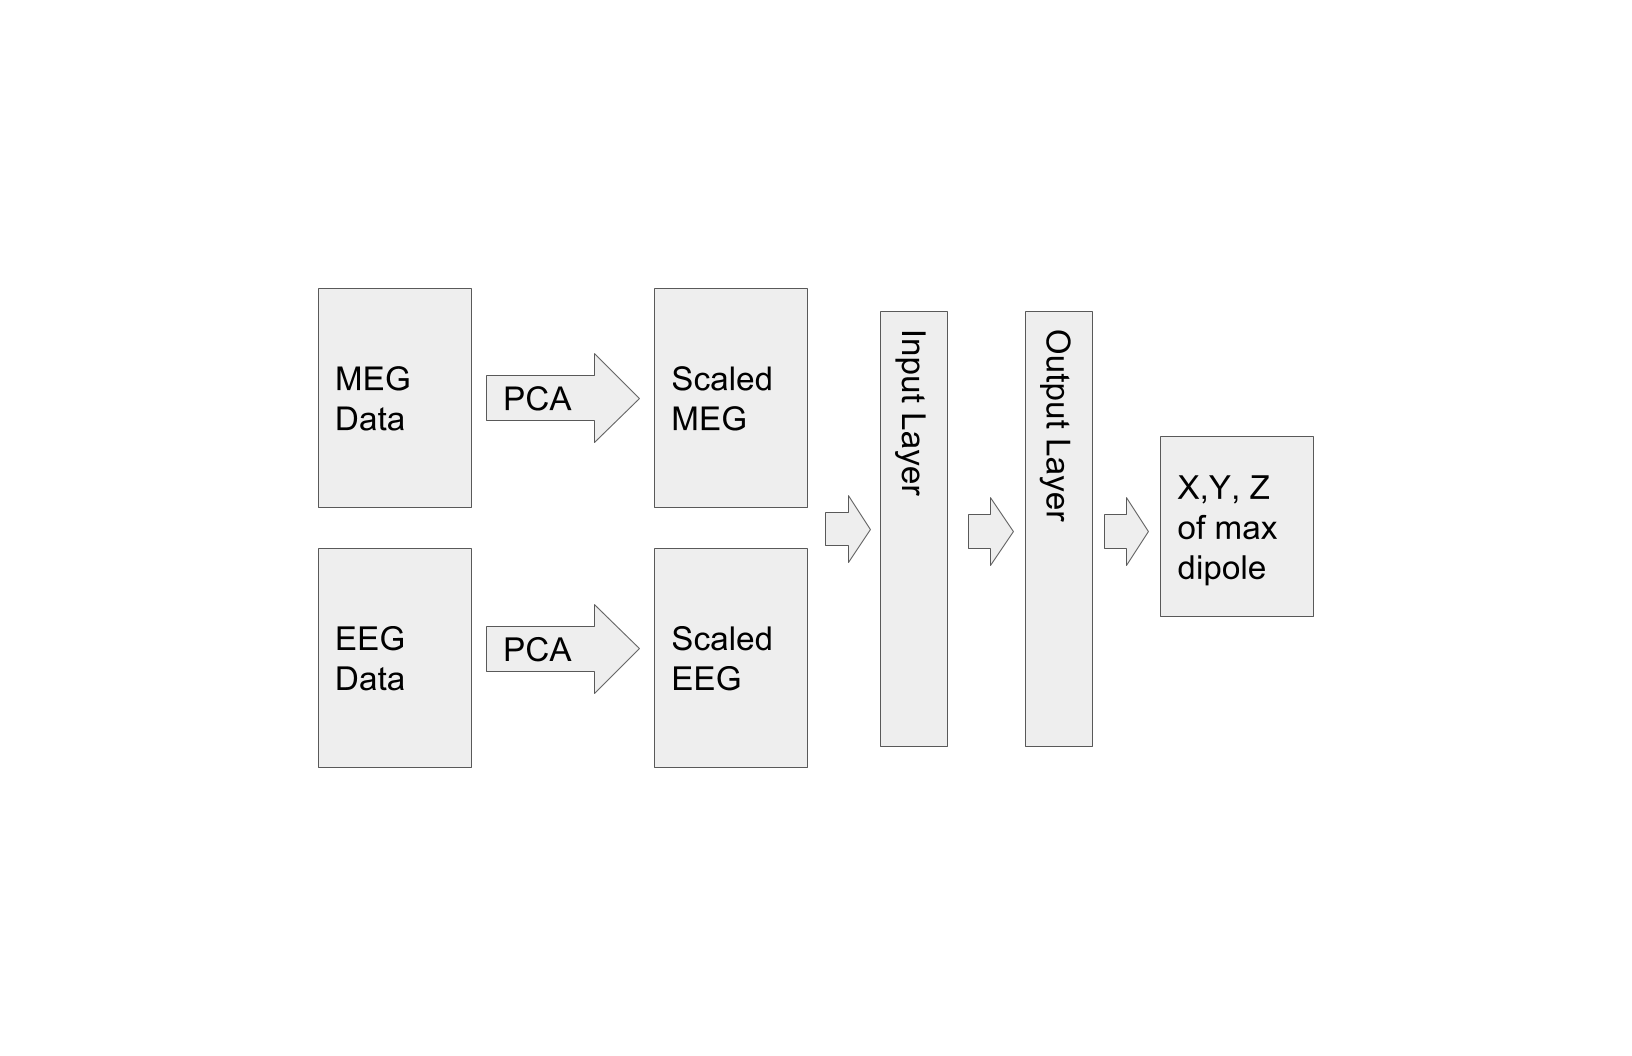
\includegraphics[width=5in]{mlp}
\caption{Block diagram of MLP neural network.}
\label{fig:mlp}
\end{figure*}

%\begin{figure*}[h!]
%\centering
%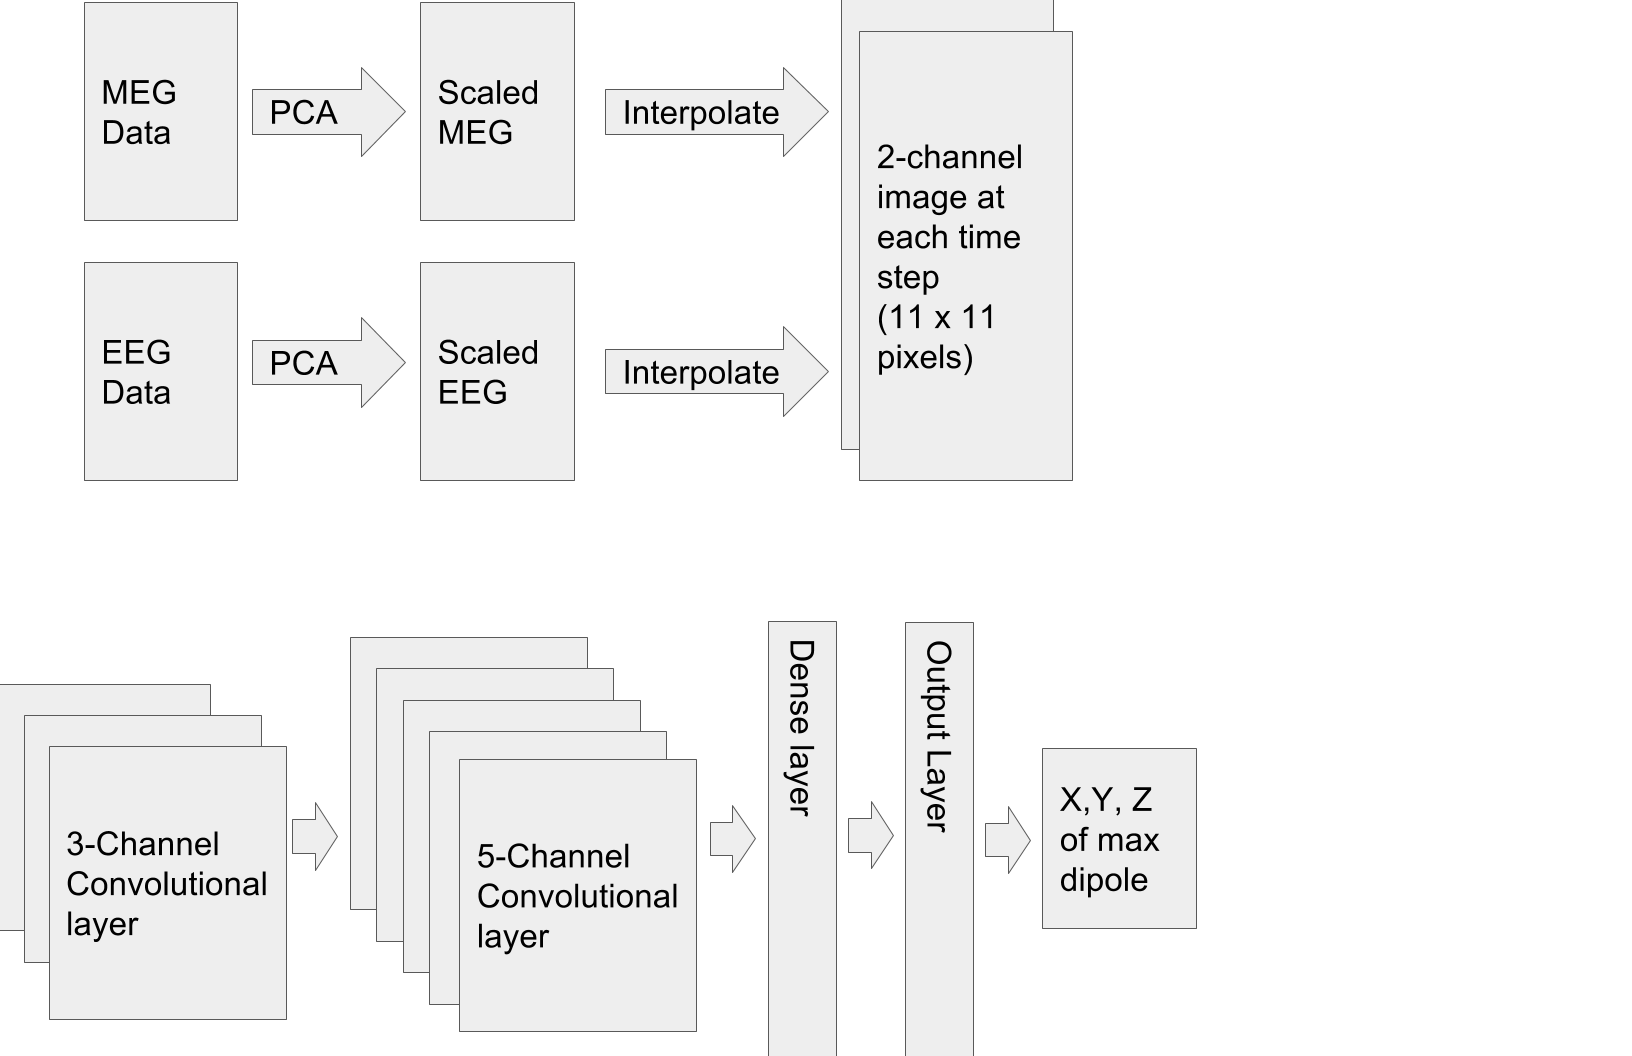
\includegraphics[width=5in]{cnn}
%\caption{Block diagram of CNN neural network.}
%\label{fig:cnn}
%\end{figure*}

%\begin{figure*}[h!]
%\centering
%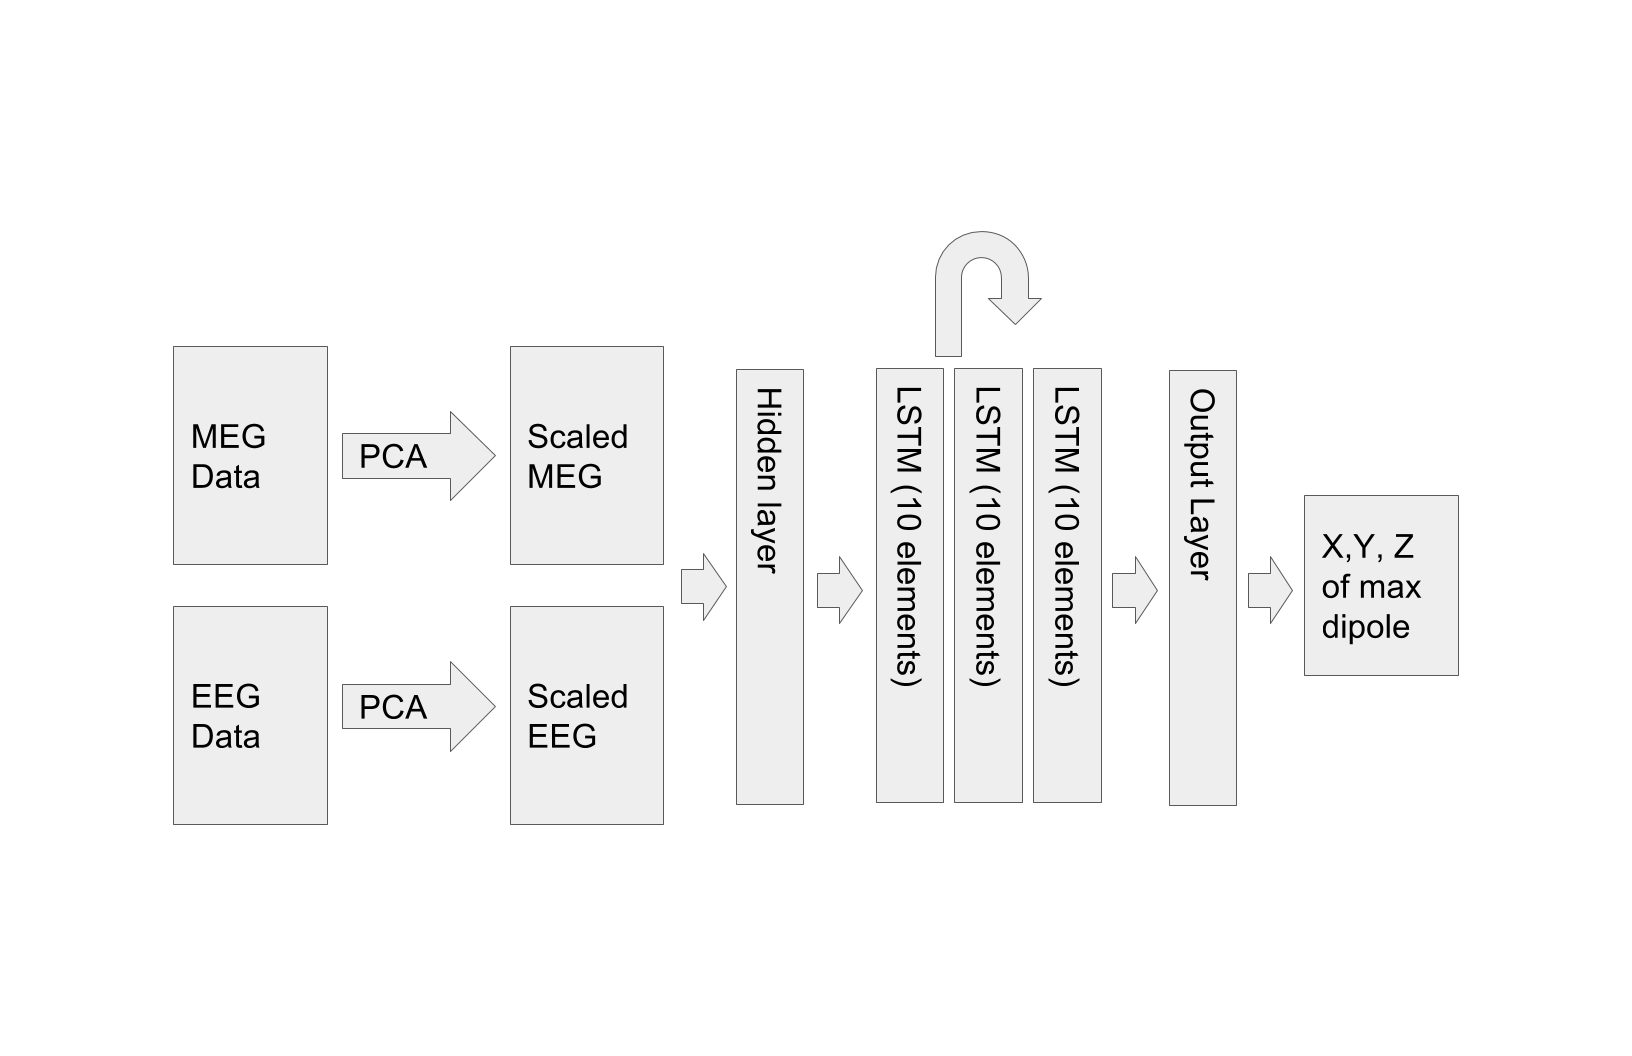
\includegraphics[width=5in]{rnn}
%\caption{Block diagram of RNN neural network.}
%\label{fig:rnn}
%\end{figure*}

\begin{figure*}[h!]
\centering
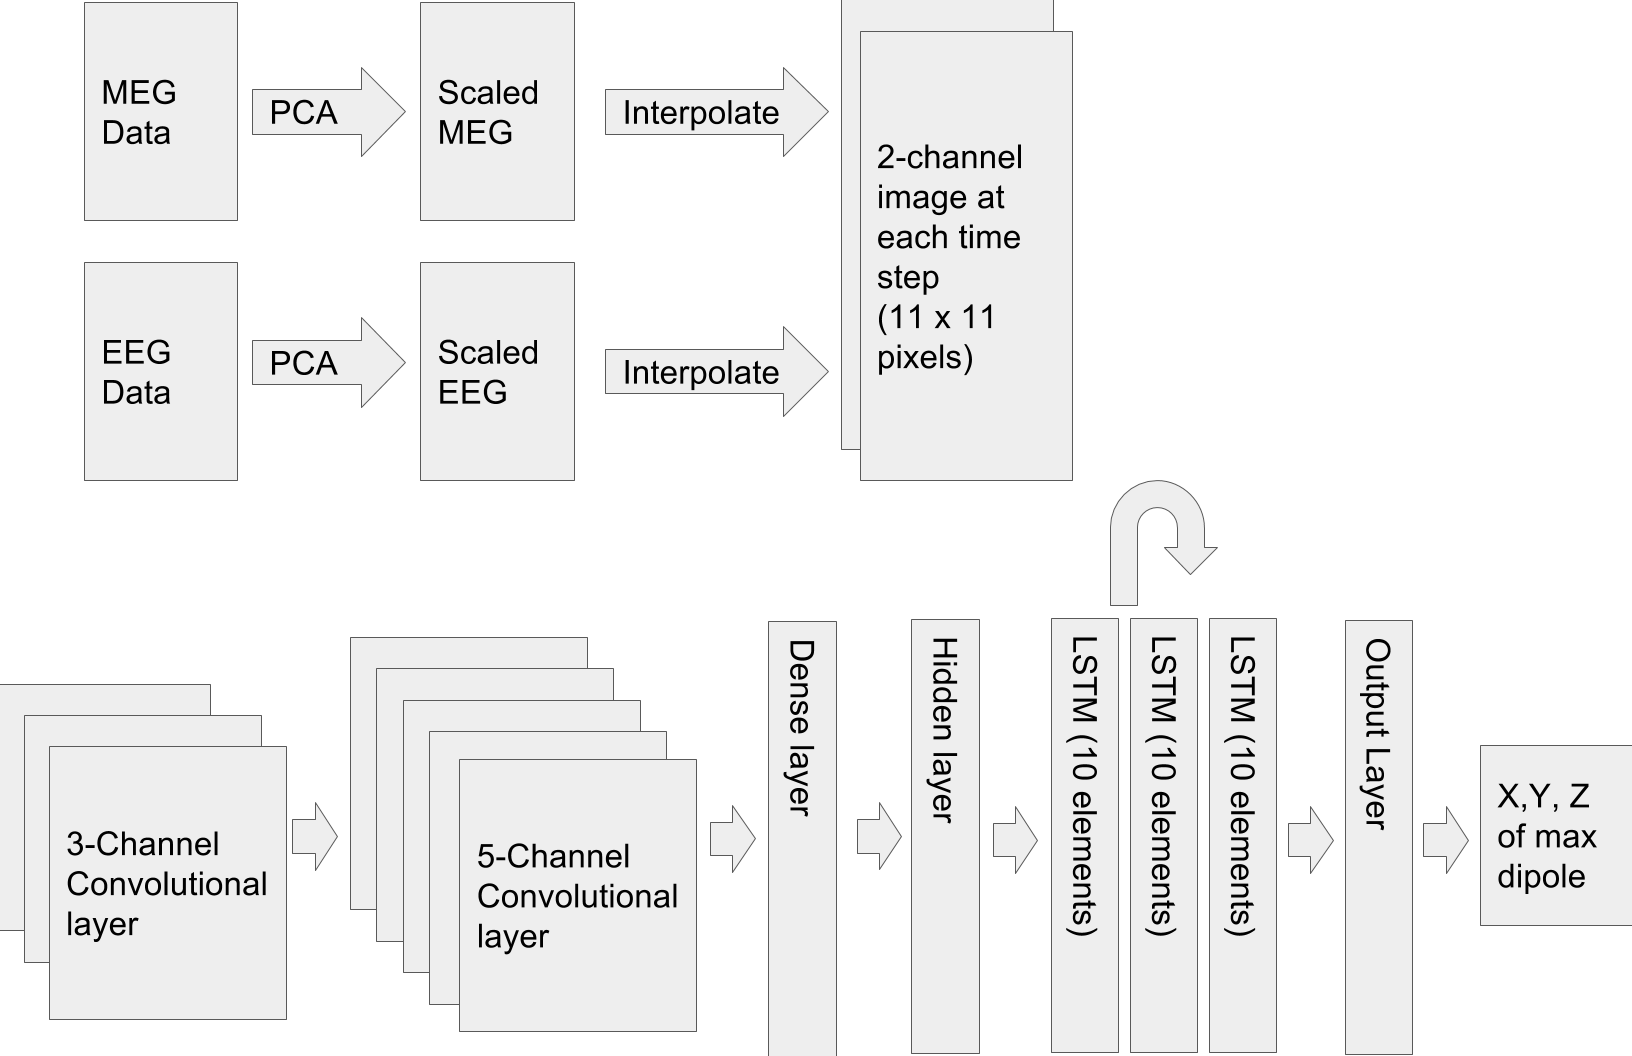
\includegraphics[width=5in]{cnnrnn}
\caption{Block diagram of CNN+RNN neural network.}
\label{fig:cnnrnn}
\end{figure*}


We considered four variations of the network structure, each of which was programmed using Google's Tensorflow API in Python (\url{tensorflow.com}). The simplest configuration was a multi-layer perceptron, where the PCA-transformed data is input as a vector at each timestep, and transformed by an input layer with ReLU activation functions, and then an output layer, with linear activation functions, to give the coordinate of the maximum current neuron at each timestep (Fig. \ref{fig:mlp}). The next network type was a convolutional neural network, where the data at each timestep was interpolated to an 11 by 11 grid, such that the data forms a sequence of 2-channel (EEG and MEG) images. The grid size was chosen such that increasing the number of pixels had no marginal benefit on the model error. There were two convolutional layers, with kernel size 3 by 3. This was followed by a dense layer which is mapped to the output with a linear activation function. We also considered a recurrent neural network, with long short term memory (LSTM) cells, with an input layer, recurrent layer, and output layer, returning the dipole location of the maximum current neuron over the entire timeseries, not at each timestep. Finally, we considered a combination of the CNN and RNN networks (Fig. \ref{fig:cnnrnn}). Network parameters are given in Table \ref{tab:params}. 

\begin{table*}[h!]
  \centering
  \begin{tabular}{c||c|c|c}
    \hline
    Network & CNN & Hidden layer & RNN\\
    \hline
    \hline
    MLP & N/A & 10 units & N/A \\
    \hline
    CNN & 2 layers (3, then 5 channels) & N/A & N/A \\
    \hline
    RNN & N/A & N/A & 10 units, 3 layers \\
    \hline
    CNN+RNN & 2 layers (3, then 5 channels) &  N/A & 10 units, 3 layers \\
  \end{tabular}
  \caption{Network parameters.}
  \label{tab:params}
\end{table*}


\subsection{Training and testing}

To train the networks, on each dataset the data was divided into randomly selected test, validation, and training sets, where the test set was 20\% of the total dataset, validation was 20\% of the remainder, and the remainder was divided into batches for training of 20\% each. Cost was the RMSE of the location of the dipole, where the true value was taken as the Minimum Norm Estimate found using the MNE Python package. Validation error was logged every 100 steps, and each batch was trained for 1250 steps (giving 5000 train steps total). We used Adam optimization to train the network parameters \cite{kingma2014adam} with a learning rate of 0.005.

\section{Results}

Training and validation curves are given in Figs. \ref{fig:aud} and \ref{fig:faces}, along with test dataset cost, for the auditory dataset and the faces dataset, respectively. For both datasets, CNN and MLP networks outperform the networks including an RNN. While they are capable of achieving low training cost, they tend to overfit, and thus do poorly on the test set (test cost of around 45 mm for the faces dataset, 30 mm for the auditory dataset). For reference, the human head is about 75 mm in diameter. On the other hand, simpler networks did better, with the CNN only network performing best (cost of 5.1 mm for the auditory set, and 1.9 mm for the faces dataset). Fewer parameters allowed for better generalization, and the CNN layer allows us to preserve spatial information critical for inversion.

The poor generalization of the RNN networks led us to suspect that it may be too sensitive to noise in the location of the peak dipole. In other words, since we were using the MNE estimate of the dipole currents as truth, and these have some inherent error due to sensor noise and inversion error, the performance of the network to estimate the location may be poor. To test this, instead of comparing the neural network estimate to the peak dipole, we instead tried comparing it to the top 100 dipoles (which is approximately the top 5\%-10\%), and picking the closest one for calculating the cost. This has the effect of averaging out error in the dipoles estimated by MNE. Plots showing the training curves for this top-100 approach are shown in Figs. \ref{fig:aud100} and \ref{fig:faces100}. Clearly, this reduces the test, training, and validation costs, but the performance ranking of the the four networks remains the same.

\begin{figure}[!t]
\centering
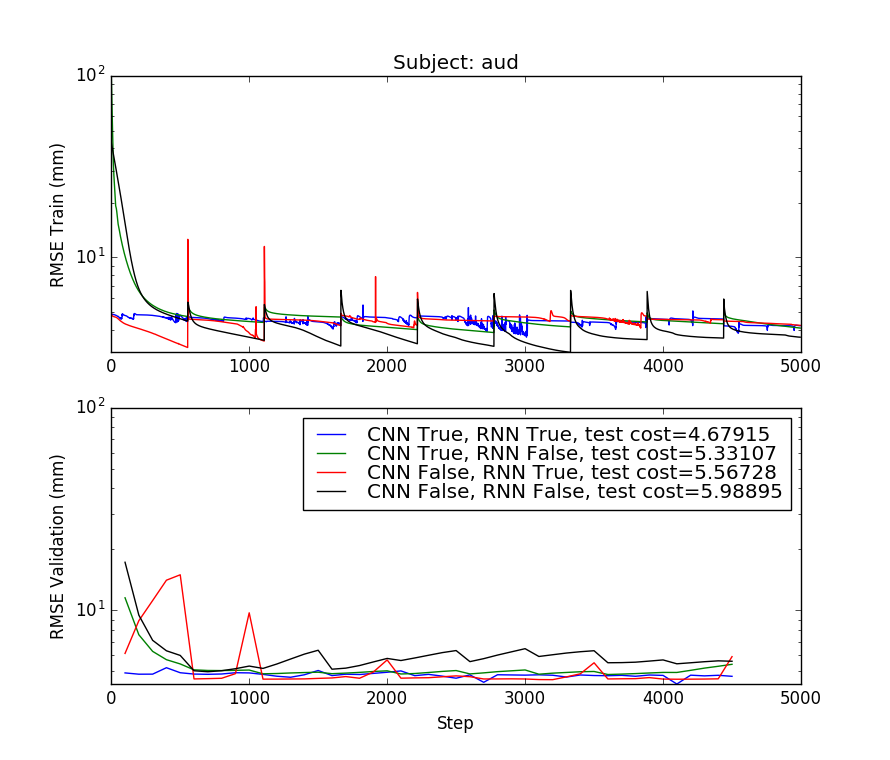
\includegraphics[width=3.5in]{aud1}
\caption{Training/validation results for auditory stimulus dataset (1 dipole).}
\label{fig:aud}
\end{figure}

\begin{figure}[!t]
\centering
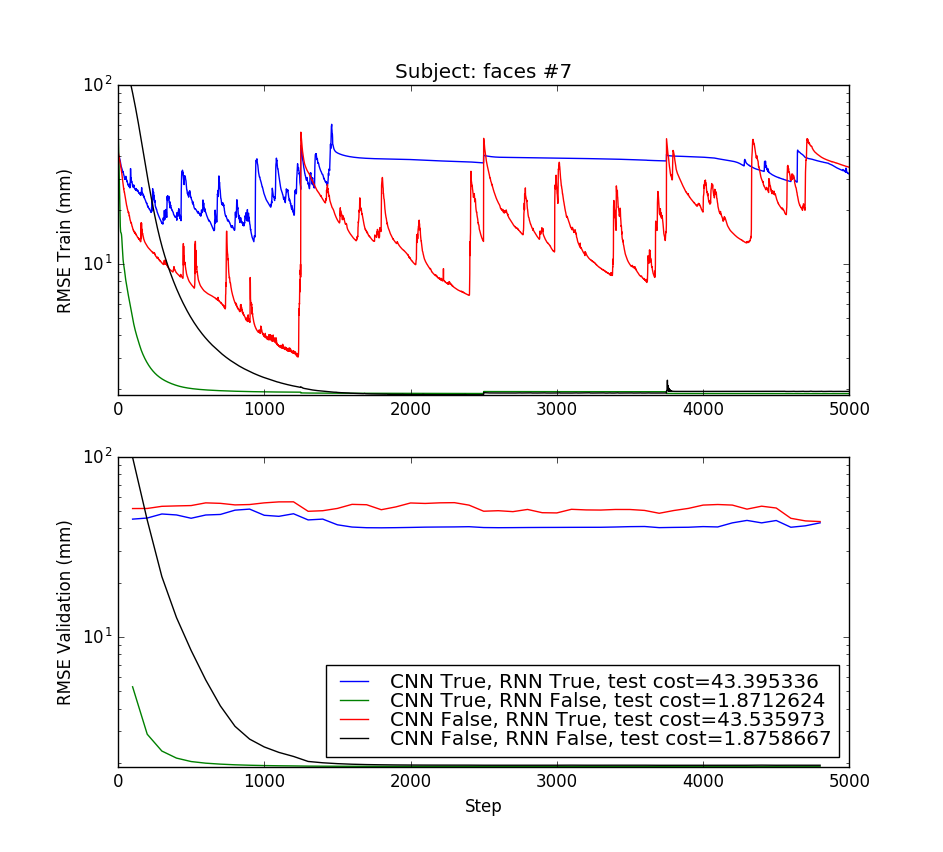
\includegraphics[width=3.5in]{faces1}
\caption{Training/validation results for faces stimulus dataset (1 dipole).}
\label{fig:faces}
\end{figure}

\begin{figure}[!t]
\centering
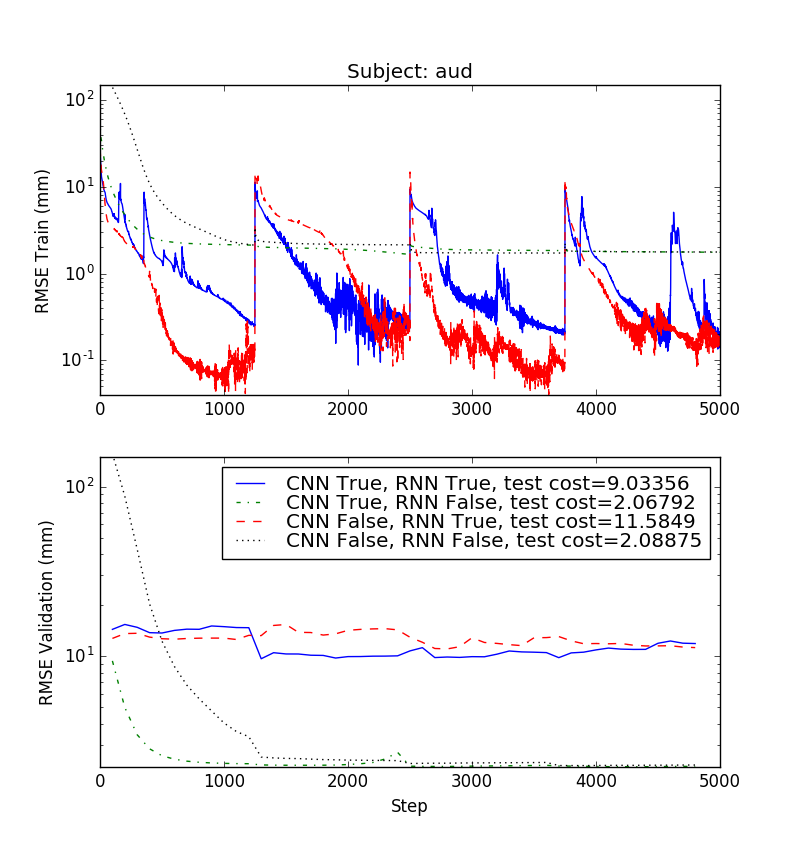
\includegraphics[width=3.5in]{aud100}
\caption{Training/validation results for auditory stimulus dataset (100 dipoles).}
\label{fig:aud100}
\end{figure}

\begin{figure}[!t]
\centering
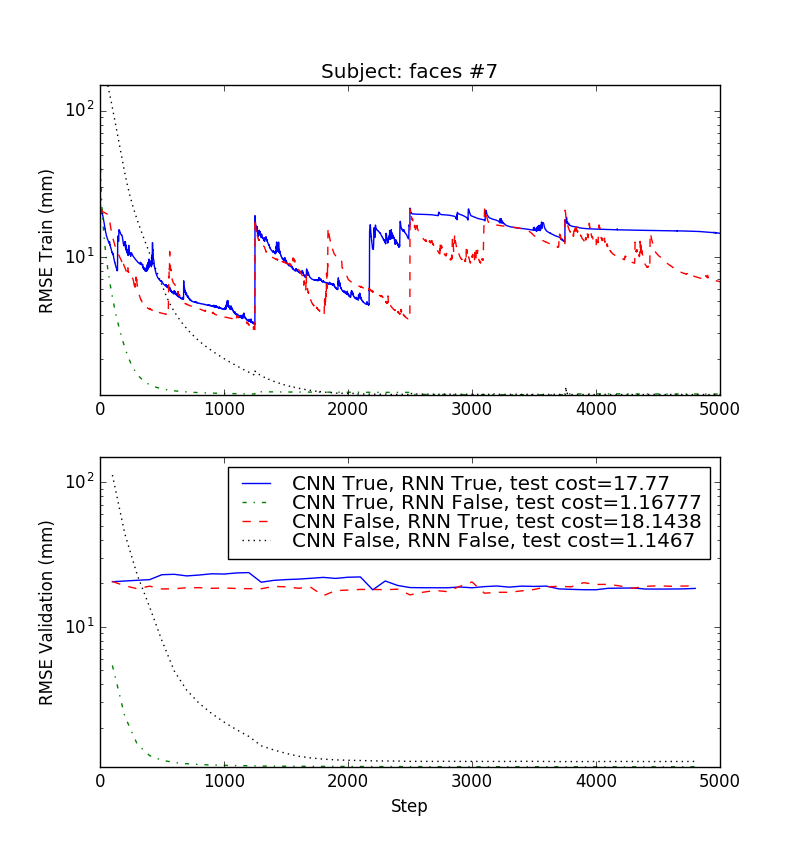
\includegraphics[width=3.5in]{faces100}
\caption{Training/validation results for faces stimulus dataset (100 dipoles).}
\label{fig:faces100}
\end{figure}

\section{Conclusion}
We have presented a new technique for rapid inversion of MEG/EEG data, using neural networks to estimate the location of the peak dipole, rather than the current distribution over the cortex. In examining four possible network architectures, it was found that the CNN networks perform best in determining the location of the peak dipole at each timestep. More complicated network architectures, or those without the CNN layers, performed worse, due to overfitting and loss of spatial information. Treating the EEG and MEG data as a two-channel image is an effective method for retaining patial field patterns, and is easily extensible to situations with more available sensors, such as NIRS. Future work may investigate using sequence-to-sequence neural machine translation to interpret timeseries.


% use section* for acknowledgment
\section*{Acknowledgment}
The authors would like to thank DARPA BAA XXX


% references section

\bibliographystyle{IEEEtran}
\bibliography{./casanova_ieee}
%\begin{IEEEbiography}[{\includegraphics[width=1in,height=1.25in,clip,keepaspectratio]{mshell}}]{Michael Shell}
% or if you just want to reserve a space for a photo:

% if you will not have a photo at all:
\begin{IEEEbiographynophoto}{Joaquin Casanova (S'05--M'09)}
  Dr. Casanova is a Research Assistant Professor in Electrical and Computer Engineering at the University of Florida. He received the B.S. and M.S. degrees in agricultural and biological engineering and the Ph.D. degree in electrical engineering from the University of Florida, Gainesville, in 2006, 2007, and 2010, respectively. His research focuses on electromagnetic sensors, machine learning, medicine, and agriculture. Dr. Casanova is a member of the American Society of Agricultural and Biological Engineers.
\end{IEEEbiographynophoto}

\begin{IEEEbiographynophoto}{Zachary D. Stoecker-Sylvia}
Mr. Stoecker-Sylvia is a computer scientist at Oceanit Laboratories, based in Honolulu, Hawaii.  He received his M.S. in computer science from Worcester Polytechnic Institute in 2004, focusing on machine learning.  His professional responsibilities involve research into artificial intelligence, machine learning, and sensor systems.  
\end{IEEEbiographynophoto}


\begin{IEEEbiographynophoto}{Ryan Y. Miyamoto}(S'97--M'03--SM'07) earned his B. S. Degree in Electro-physics from Tokyo Institute of Technology in 1997, M.S. and Ph.D. degree from the University of California, Los Angeles in 1999 and 2002, respectively. Dr. Miyamoto is the Director of Electronic Systems at Oceanit in Honolulu, HI. He is responsible for Oceanit’s RF programs including electronic warfare, wireless communications and RF sensors. 
     He has authored and co-authored more than 30 journal and conference papers. Dr. Miyamoto received the MTT-S Outstanding Young Engineer Award in 2012. He was a recipient of the ISAP award presented at 2000 International Symposium on Antennas and Propagation in Fukuoka, Japan. He was the Technical Program Co-Chair for 2017 IEEE International Microwave Symposium (IMS).
  
\end{IEEEbiographynophoto}

\begin{IEEEbiographynophoto}{Jenshan Lin}(S'91--M'94--SM'00--F'10) received the Ph.D. degree in electrical engineering from the University of California, Los Angeles, CA, USA, in 1994.
  He was with Lucent Bell Labs, Murray Hill, NJ, USA, from 1994 to 2001, and Agere Systems, Holmdel, NJ, USA, a spin-off company of Lucent Bell Labs, from 2001 to 2003. In 2003, he joined the University of Florida, Gainesville, FL, USA, where he is currently a Professor. Since October 2016, he has been on assignment to work for the U.S. National Science Foundation as a Program Director in Communications, Circuits, and Sensing Systems (CCSS) Program. He has authored or coauthored over 260 technical publications in refereed journals and conference proceedings. He holds 15 U.S. patents. His current research interests include sensors and biomedical applications of microwave and millimeter-wave technologies, wireless power transfer, and wireless communication systems.

Dr. Lin was a recipient of the 1994 UCLA Outstanding Ph.D. Award, the 1997 Eta Kappa Nu Outstanding Young Electrical Engineer Honorable Mention Award, the 2007 IEEE Microwave Theory and Techniques Society (MTT-S) N. Walter Cox Award, the 2015 IEEE Wireless Power Transfer Conference Best Paper Award, the 2016 Distinguished Alumnus Award from National Chiao Tung University, Hsinchu, Taiwan, and the 2016 IEEE RFIC Symposium Tina Quach Outstanding Service Award. He was the General Chair of the 2008 RFIC Symposium, the Technical Program Chair of the 2009 Radio and Wireless Symposium, and the General Co-Chair of the 2012 Asia–Pacific Microwave Conference. He served as the Editor-in-Chief of the IEEE TRANSACTIONS ON MICROWAVE THEORY AND TECHNIQUES in 2014-2016.
  
\end{IEEEbiographynophoto}



% that's all folks
\end{document}


\grid
